%% Kortsett fra mattelab.no – laget automatisk av bygg.py. Rediger gjerne til eget bruk.
%% Kompiler med lualatex.
\documentclass[11pt,a4paper]{article}
\usepackage[norsk]{babel}
\usepackage[a4paper,margin=1.2cm,bottom=1.7cm]{geometry}
\usepackage{fontspec}
\usepackage{unicode-math}
\setmainfont{TeX Gyre Pagella}
\setsansfont{TeX Gyre Heros}[Scale=MatchLowercase]
\setmathfont{TeX Gyre Pagella Math}
\usepackage{xcolor}
\definecolor{blekk}{HTML}{16213A}
\definecolor{dempet}{HTML}{566077}
\definecolor{m1}{HTML}{2F4AB0}
\usepackage{tikz}
\usepackage{qrcode}
\usepackage{fancyhdr}
\usepackage[hidelinks]{hyperref}
\pdfvariable suppressoptionalinfo \numexpr 1+2+4+8+16+32+64+128+256+512\relax
\setlength{\parindent}{0pt}
\setlength{\parskip}{0pt}
\pagestyle{fancy}
\fancyhf{}
\renewcommand{\headrulewidth}{0pt}
\fancyfoot[L]{\sffamily\footnotesize\color{dempet}mattelab.no · Funksjon, utregning og svar · kortsett K15}
\fancyfoot[R]{\sffamily\footnotesize\color{dempet}Side \thepage}
\begin{document}
\begin{minipage}[t]{0.8\linewidth}\vspace{0pt}
{\sffamily\small\color{dempet}Kortsett K15 · R1 · mattelab.no}\par\vspace{0.25em}
{\fontsize{20}{24}\selectfont\bfseries Funksjon, utregning og svar}\par\vspace{0.5em}
Finn tre og tre kort som hører sammen: en funksjon, utregningen av den deriverte med en regel, og den forenklede deriverte. Skriv ved hver gruppe hvilken regel som er brukt.\par\vspace{0.4em}{\small\color{dempet}Klipp langs de stiplede linjene. Koden nede i hjørnet (K15-01, K15-02, …) viser hvilket sett kortet hører til.}
\end{minipage}\hfill
\begin{minipage}[t]{0.15\linewidth}\vspace{0pt}\raggedleft
\qrcode[height=1.9cm]{https://mattelab.no/varierende/funksjon-utregning-svar.html}
\end{minipage}\par\vspace{0.8em}

\noindent\begin{tikzpicture}
\useasboundingbox (0,0) rectangle (6.19,4.0);
\node[text width=5.29cm, align=center, font=\Large] at (3.095,2.08) {$f(x) = \ln(x^2 + 1)$};
\draw[black!45, line width=0.4pt, dash pattern=on 3pt off 2.5pt] (0,0) rectangle (6.19,4.0);
\node[anchor=south east, font=\sffamily\scriptsize, text=black!55, inner sep=0pt] at (6.04,0.14) {K15-01};
\end{tikzpicture}%
\begin{tikzpicture}
\useasboundingbox (0,0) rectangle (6.19,4.0);
\node[text width=5.29cm, align=center, font=\Large] at (3.095,2.08) {$f'(x) = 2x \cdot e^x + x^2 \cdot e^x$};
\draw[black!45, line width=0.4pt, dash pattern=on 3pt off 2.5pt] (0,0) rectangle (6.19,4.0);
\node[anchor=south east, font=\sffamily\scriptsize, text=black!55, inner sep=0pt] at (6.04,0.14) {K15-02};
\end{tikzpicture}%
\begin{tikzpicture}
\useasboundingbox (0,0) rectangle (6.19,4.0);
\node[text width=5.29cm, align=center, font=\Large] at (3.095,2.08) {$f(x) = \dfrac{x}{x + 1}$};
\draw[black!45, line width=0.4pt, dash pattern=on 3pt off 2.5pt] (0,0) rectangle (6.19,4.0);
\node[anchor=south east, font=\sffamily\scriptsize, text=black!55, inner sep=0pt] at (6.04,0.14) {K15-03};
\end{tikzpicture}%
\par\nointerlineskip
\noindent\begin{tikzpicture}
\useasboundingbox (0,0) rectangle (6.19,4.0);
\node[text width=5.29cm, align=center, font=\Large] at (3.095,2.08) {$f'(x) = 6(2x + 1)^2$};
\draw[black!45, line width=0.4pt, dash pattern=on 3pt off 2.5pt] (0,0) rectangle (6.19,4.0);
\node[anchor=south east, font=\sffamily\scriptsize, text=black!55, inner sep=0pt] at (6.04,0.14) {K15-04};
\end{tikzpicture}%
\begin{tikzpicture}
\useasboundingbox (0,0) rectangle (6.19,4.0);
\node[text width=5.29cm, align=center, font=\Large] at (3.095,2.08) {$f(x) = \dfrac{e^x}{x}$};
\draw[black!45, line width=0.4pt, dash pattern=on 3pt off 2.5pt] (0,0) rectangle (6.19,4.0);
\node[anchor=south east, font=\sffamily\scriptsize, text=black!55, inner sep=0pt] at (6.04,0.14) {K15-05};
\end{tikzpicture}%
\begin{tikzpicture}
\useasboundingbox (0,0) rectangle (6.19,4.0);
\node[text width=5.29cm, align=center, font=\Large] at (3.095,2.08) {$f'(x) = x(x + 2)e^x$};
\draw[black!45, line width=0.4pt, dash pattern=on 3pt off 2.5pt] (0,0) rectangle (6.19,4.0);
\node[anchor=south east, font=\sffamily\scriptsize, text=black!55, inner sep=0pt] at (6.04,0.14) {K15-06};
\end{tikzpicture}%
\par\nointerlineskip
\noindent\begin{tikzpicture}
\useasboundingbox (0,0) rectangle (6.19,4.0);
\node[text width=5.29cm, align=center, font=\Large] at (3.095,2.08) {$f'(x) = \dfrac{1}{x^2 + 1} \cdot 2x$};
\draw[black!45, line width=0.4pt, dash pattern=on 3pt off 2.5pt] (0,0) rectangle (6.19,4.0);
\node[anchor=south east, font=\sffamily\scriptsize, text=black!55, inner sep=0pt] at (6.04,0.14) {K15-07};
\end{tikzpicture}%
\begin{tikzpicture}
\useasboundingbox (0,0) rectangle (6.19,4.0);
\node[text width=5.29cm, align=center, font=\Large] at (3.095,2.08) {$f(x) = x^2 e^x$};
\draw[black!45, line width=0.4pt, dash pattern=on 3pt off 2.5pt] (0,0) rectangle (6.19,4.0);
\node[anchor=south east, font=\sffamily\scriptsize, text=black!55, inner sep=0pt] at (6.04,0.14) {K15-08};
\end{tikzpicture}%
\begin{tikzpicture}
\useasboundingbox (0,0) rectangle (6.19,4.0);
\node[text width=5.29cm, align=center, font=\Large] at (3.095,2.08) {$f'(x) = \dfrac{1 \cdot (x + 1) - x \cdot 1}{(x + 1)^2}$};
\draw[black!45, line width=0.4pt, dash pattern=on 3pt off 2.5pt] (0,0) rectangle (6.19,4.0);
\node[anchor=south east, font=\sffamily\scriptsize, text=black!55, inner sep=0pt] at (6.04,0.14) {K15-09};
\end{tikzpicture}%
\par\nointerlineskip
\noindent\begin{tikzpicture}
\useasboundingbox (0,0) rectangle (6.19,4.0);
\node[text width=5.29cm, align=center, font=\Large] at (3.095,2.08) {$f'(x) = 1 \cdot \ln x + x \cdot \dfrac{1}{x}$};
\draw[black!45, line width=0.4pt, dash pattern=on 3pt off 2.5pt] (0,0) rectangle (6.19,4.0);
\node[anchor=south east, font=\sffamily\scriptsize, text=black!55, inner sep=0pt] at (6.04,0.14) {K15-10};
\end{tikzpicture}%
\begin{tikzpicture}
\useasboundingbox (0,0) rectangle (6.19,4.0);
\node[text width=5.29cm, align=center, font=\Large] at (3.095,2.08) {$f'(x) = -2x e^{-x^2}$};
\draw[black!45, line width=0.4pt, dash pattern=on 3pt off 2.5pt] (0,0) rectangle (6.19,4.0);
\node[anchor=south east, font=\sffamily\scriptsize, text=black!55, inner sep=0pt] at (6.04,0.14) {K15-11};
\end{tikzpicture}%
\begin{tikzpicture}
\useasboundingbox (0,0) rectangle (6.19,4.0);
\node[text width=5.29cm, align=center, font=\Large] at (3.095,2.08) {$f'(x) = e^{-x^2} \cdot (-2x)$};
\draw[black!45, line width=0.4pt, dash pattern=on 3pt off 2.5pt] (0,0) rectangle (6.19,4.0);
\node[anchor=south east, font=\sffamily\scriptsize, text=black!55, inner sep=0pt] at (6.04,0.14) {K15-12};
\end{tikzpicture}%
\par\nointerlineskip
\noindent\begin{tikzpicture}
\useasboundingbox (0,0) rectangle (6.19,4.0);
\node[text width=5.29cm, align=center, font=\Large] at (3.095,2.08) {$f'(x) = \dfrac{(x - 1)e^x}{x^2}$};
\draw[black!45, line width=0.4pt, dash pattern=on 3pt off 2.5pt] (0,0) rectangle (6.19,4.0);
\node[anchor=south east, font=\sffamily\scriptsize, text=black!55, inner sep=0pt] at (6.04,0.14) {K15-13};
\end{tikzpicture}%
\begin{tikzpicture}
\useasboundingbox (0,0) rectangle (6.19,4.0);
\node[text width=5.29cm, align=center, font=\Large] at (3.095,2.08) {$f'(x) = \dfrac{1}{(x + 1)^2}$};
\draw[black!45, line width=0.4pt, dash pattern=on 3pt off 2.5pt] (0,0) rectangle (6.19,4.0);
\node[anchor=south east, font=\sffamily\scriptsize, text=black!55, inner sep=0pt] at (6.04,0.14) {K15-14};
\end{tikzpicture}%
\begin{tikzpicture}
\useasboundingbox (0,0) rectangle (6.19,4.0);
\node[text width=5.29cm, align=center, font=\Large] at (3.095,2.08) {$f'(x) = 3(2x + 1)^2 \cdot 2$};
\draw[black!45, line width=0.4pt, dash pattern=on 3pt off 2.5pt] (0,0) rectangle (6.19,4.0);
\node[anchor=south east, font=\sffamily\scriptsize, text=black!55, inner sep=0pt] at (6.04,0.14) {K15-15};
\end{tikzpicture}%
\par\nointerlineskip
\noindent\begin{tikzpicture}
\useasboundingbox (0,0) rectangle (6.19,4.0);
\node[text width=5.29cm, align=center, font=\Large] at (3.095,2.08) {$f(x) = (2x + 1)^3$};
\draw[black!45, line width=0.4pt, dash pattern=on 3pt off 2.5pt] (0,0) rectangle (6.19,4.0);
\node[anchor=south east, font=\sffamily\scriptsize, text=black!55, inner sep=0pt] at (6.04,0.14) {K15-16};
\end{tikzpicture}%
\begin{tikzpicture}
\useasboundingbox (0,0) rectangle (6.19,4.0);
\node[text width=5.29cm, align=center, font=\Large] at (3.095,2.08) {$f(x) = e^{-x^2}$};
\draw[black!45, line width=0.4pt, dash pattern=on 3pt off 2.5pt] (0,0) rectangle (6.19,4.0);
\node[anchor=south east, font=\sffamily\scriptsize, text=black!55, inner sep=0pt] at (6.04,0.14) {K15-17};
\end{tikzpicture}%
\begin{tikzpicture}
\useasboundingbox (0,0) rectangle (6.19,4.0);
\node[text width=5.29cm, align=center, font=\Large] at (3.095,2.08) {$f'(x) = \dfrac{e^x \cdot x - e^x \cdot 1}{x^2}$};
\draw[black!45, line width=0.4pt, dash pattern=on 3pt off 2.5pt] (0,0) rectangle (6.19,4.0);
\node[anchor=south east, font=\sffamily\scriptsize, text=black!55, inner sep=0pt] at (6.04,0.14) {K15-18};
\end{tikzpicture}%
\par\nointerlineskip
\noindent\begin{tikzpicture}
\useasboundingbox (0,0) rectangle (6.19,4.0);
\node[text width=5.29cm, align=center, font=\Large] at (3.095,2.08) {$f(x) = x \ln x$};
\draw[black!45, line width=0.4pt, dash pattern=on 3pt off 2.5pt] (0,0) rectangle (6.19,4.0);
\node[anchor=south east, font=\sffamily\scriptsize, text=black!55, inner sep=0pt] at (6.04,0.14) {K15-19};
\end{tikzpicture}%
\begin{tikzpicture}
\useasboundingbox (0,0) rectangle (6.19,4.0);
\node[text width=5.29cm, align=center, font=\Large] at (3.095,2.08) {$f'(x) = \ln x + 1$};
\draw[black!45, line width=0.4pt, dash pattern=on 3pt off 2.5pt] (0,0) rectangle (6.19,4.0);
\node[anchor=south east, font=\sffamily\scriptsize, text=black!55, inner sep=0pt] at (6.04,0.14) {K15-20};
\end{tikzpicture}%
\begin{tikzpicture}
\useasboundingbox (0,0) rectangle (6.19,4.0);
\node[text width=5.29cm, align=center, font=\Large] at (3.095,2.08) {$f'(x) = \dfrac{2x}{x^2 + 1}$};
\draw[black!45, line width=0.4pt, dash pattern=on 3pt off 2.5pt] (0,0) rectangle (6.19,4.0);
\node[anchor=south east, font=\sffamily\scriptsize, text=black!55, inner sep=0pt] at (6.04,0.14) {K15-21};
\end{tikzpicture}%
\par\nointerlineskip
\noindent\begin{tikzpicture}
\useasboundingbox (0,0) rectangle (6.19,4.0);
\node[anchor=south east, font=\sffamily\scriptsize, text=black!40, inner sep=0pt] at (6.04,0.14) {Eget kort};
\draw[black!45, line width=0.4pt, dash pattern=on 3pt off 2.5pt] (0,0) rectangle (6.19,4.0);
\end{tikzpicture}%
\begin{tikzpicture}
\useasboundingbox (0,0) rectangle (6.19,4.0);
\node[anchor=south east, font=\sffamily\scriptsize, text=black!40, inner sep=0pt] at (6.04,0.14) {Eget kort};
\draw[black!45, line width=0.4pt, dash pattern=on 3pt off 2.5pt] (0,0) rectangle (6.19,4.0);
\end{tikzpicture}%
\begin{tikzpicture}
\useasboundingbox (0,0) rectangle (6.19,4.0);
\node[anchor=south east, font=\sffamily\scriptsize, text=black!40, inner sep=0pt] at (6.04,0.14) {Eget kort};
\draw[black!45, line width=0.4pt, dash pattern=on 3pt off 2.5pt] (0,0) rectangle (6.19,4.0);
\end{tikzpicture}%
\par\nointerlineskip
\end{document}
